\chapter{Разработка решения}

\section{Общая концепция решения}

Описание общей концепции разрабатываемого решения.

\section{Архитектура решения}

Описание архитектуры решения с использованием диаграмм.

\begin{figure}[H]
\centering
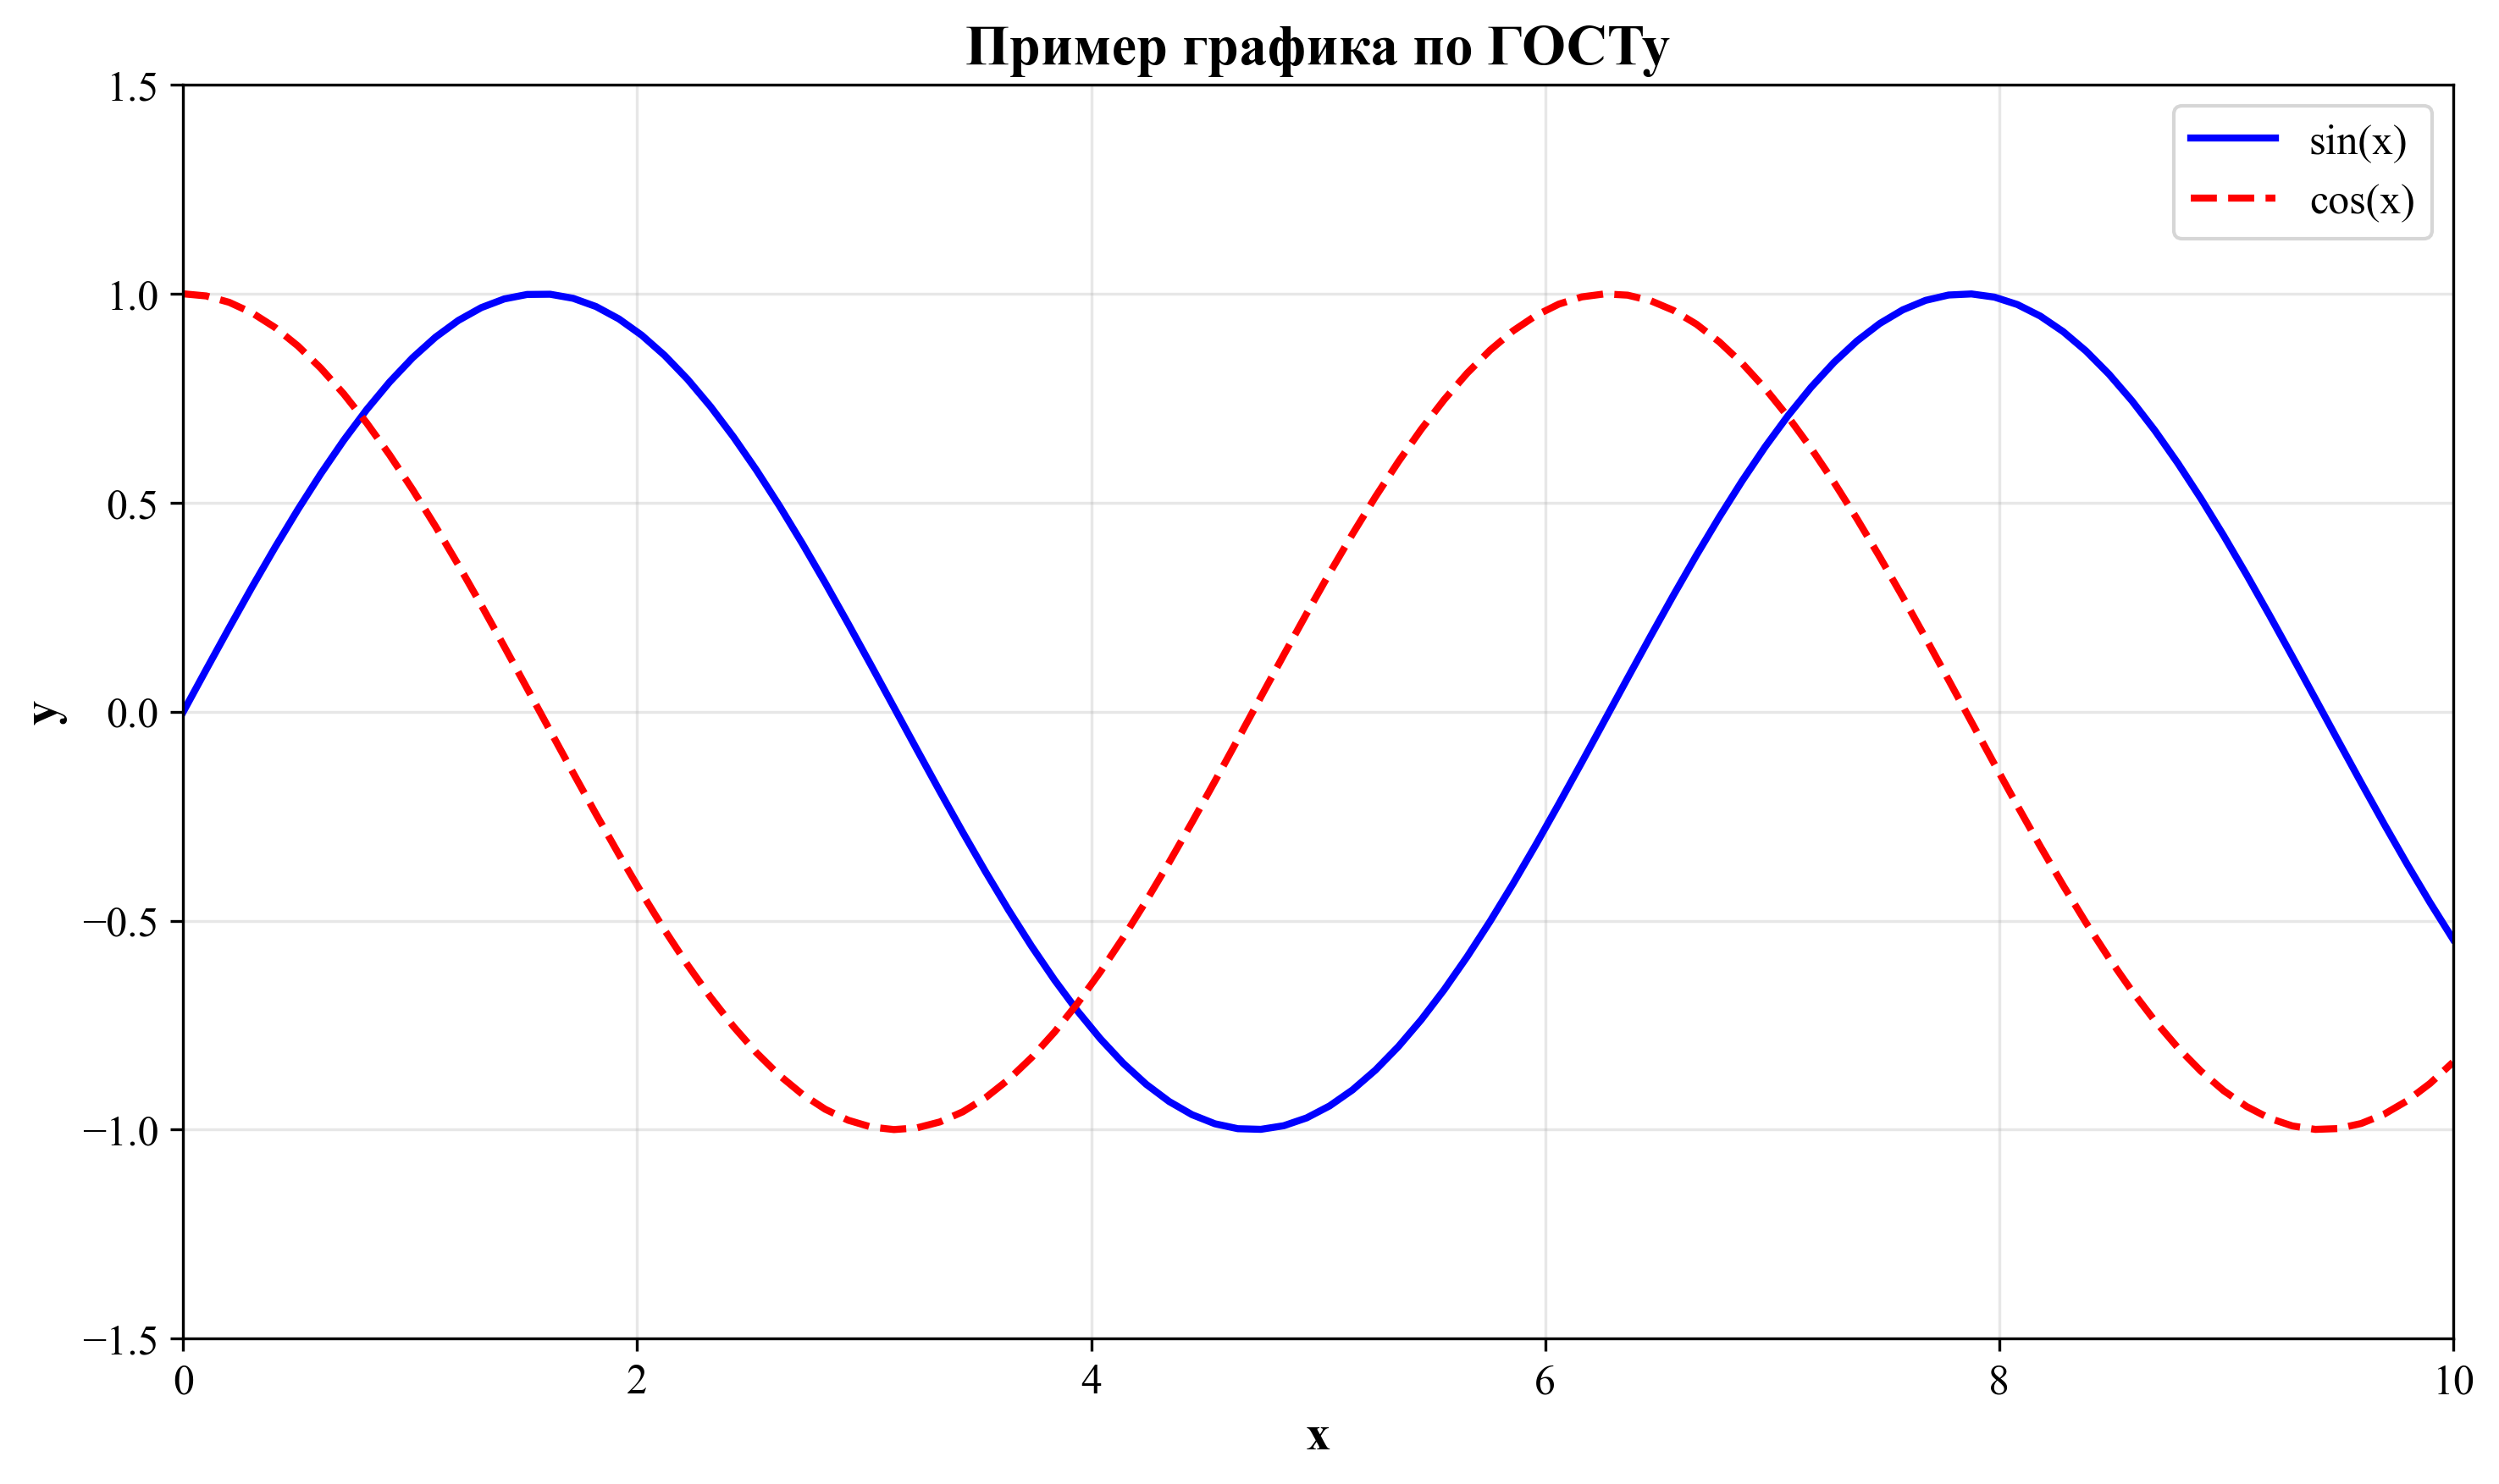
\includegraphics[width=0.9\textwidth]{images/example_plot.png}
\caption{Общая архитектура системы}
\label{fig:system_architecture}
\end{figure}

На рисунке \ref{fig:system_architecture} представлена общая архитектура разрабатываемой системы, включающая основные компоненты и их взаимодействие.

\begin{table}[H]
\centering
\caption{Технические характеристики компонентов}
\label{tab:component_specs}
\begin{tabular}{|l|c|c|c|}
\hline
\textbf{Компонент} & \textbf{Производительность} & \textbf{Память} & \textbf{Время отклика} \\
\hline
Веб-сервер & 1000 RPS & 512 MB & 50 мс \\
База данных & 500 запросов/с & 1 GB & 10 мс \\
Кэш & 10000 операций/с & 256 MB & 1 мс \\
API Gateway & 2000 RPS & 128 MB & 5 мс \\
\hline
\end{tabular}
\end{table}

В таблице \ref{tab:component_specs} приведены технические характеристики основных компонентов системы.

\begin{equation}
P(x) = \frac{e^{x_i}}{\sum_{j=1}^{n} e^{x_j}}
\label{eq:softmax}
\end{equation}

Формула \ref{eq:softmax} описывает функцию softmax, используемую для нормализации вероятностей.

\begin{lstlisting}[style=code, language=Python, caption={Пример реализации API}, label={lst:api_implementation}]
from flask import Flask, request, jsonify
import numpy as np

app = Flask(__name__)

@app.route('/predict', methods=['POST'])
def predict():
    """API endpoint for predictions"""
    data = request.get_json()
    
    # Process input data
    features = np.array(data['features'])
    
    # Make prediction
    prediction = model.predict(features)
    
    return jsonify({
        'prediction': prediction.tolist(),
        'confidence': float(np.max(prediction))
    })

if __name__ == '__main__':
    app.run(debug=True)
\end{lstlisting}

В листинге \ref{lst:api_implementation} показана реализация API endpoint для получения предсказаний от модели машинного обучения.

\subsection{Общая архитектура}

Описание общей архитектуры системы.

\subsection{Компоненты системы}

Описание основных компонентов системы.

\section{Алгоритмы и методы}

Описание используемых алгоритмов и методов.

\subsection{Алгоритм 1}

Описание первого алгоритма.

\begin{algorithm}
\caption{Название алгоритма}
\begin{algorithmic}[1]
\STATE Инициализация
\WHILE{условие}
    \STATE Действие 1
    \STATE Действие 2
\ENDWHILE
\RETURN результат
\end{algorithmic}
\end{algorithm}

\subsection{Алгоритм 2}

Описание второго алгоритма.

\section{Реализация}

Описание процесса реализации решения.

\subsection{Выбор технологий}

Обоснование выбора используемых технологий.

\subsection{Структура проекта}

Описание структуры программного проекта.

\section{Выводы по главе}

Краткие выводы по разработанному решению.
